%% Submissions for peer-review must enable line-numbering 
%% using the lineno option in the \documentclass command.
\documentclass[fleqn,10pt,lineno]{wlpeerj}
\usepackage{algorithm}
\usepackage{algpseudocode}

\title{A Cluster-Conditioned Explainable AI Framework for Interpretable 
Decision Support: Surrogate Rule Extraction for Agricultural 
Training Allocation}

\author[1]{Kitti Chiewchan}
\author[2]{Jumtip Seneerattanaprayul}
\affil[1]{Computer Education Program, Faculty of Education, Bansomdejchaopraya Rajabhat University, Bangkok, Thailand}
\affil[2]{Department of Agricultural and Resource Economics, Faculty of Economics, Kasetsart University, Bangkok, Thailand}
\corrauthor[1]{Kitti Chiewchan}{kitti.ch@bsru.ac.th}

\begin{abstract}
Allocating training programs to farmers with different backgrounds requires transparent methods that explain which farmer characteristics 
lead to better learning outcomes. We propose SAR (Segment--Attribute--Recommend), a systems architecture for targeted resource allocation. SAR combines three stages: 
(1) grouping farmers into segments based on their profiles, (2) identifying the key characteristics within each segment, and (3) converting these findings 
into simple IF--THEN decision rules for practical use.

We test SAR on agricultural training outcomes using data from $n=833$ farmers in Thailand's Smart Farmer program. 
The system identifies three farmer segments with different drivers of skill improvement: baseline experience,
 production management capability, and educational background. The extracted decision rules achieve 91.4\% 
 accuracy on held-out test data, 95.3\% $\pm$ 2.5\% cross-validated accuracy, and 93.3\% accuracy on the full dataset.

SAR offers a transparent, auditable framework for targeted resource allocation in agriculture and policy settings. 
Unlike black-box algorithms, SAR produces human-readable rules that non-technical administrators can apply without 
machine learning expertise.
\end{abstract}

%% \textbf{Keywords:} Explainable AI (XAI); Surrogate Modeling; Machine Learning; Agricultural Extension; Decision Support Systems; Farmer Segmentation

\begin{document}

\flushbottom
\maketitle
\thispagestyle{empty}

\section*{Introduction}

Providing agricultural training that meets the needs of every farmer is a major challenge. 
Most national programs still use the same curriculum for everyone, regardless of a farmer’s skill level or background. 
This "one-size-fits-all" approach often leads to wasted resources and poor learning outcomes, 
as many farmers struggle to adopt new practices. To improve results, we need a better way to match 
training programs to a farmer’s specific skills, risks, and resources.

While machine learning can predict outcomes, using it for policy decisions requires transparency.
 Public sector decision-makers must be able to justify every recommendation, which makes black-box models unsuitable. 
 Furthermore, effective resource allocation requires knowing not just what will happen, 
 but why certain farmer characteristics lead to different results.

Explainable AI (XAI), specifically SHAP (SHapley Additive exPlanations), helps us see which factors influence a model’s predictions.
 However, current XAI research in agriculture often has two limitations. 
 First, studies often stop at creating charts and do not turn these insights into clear rules that practitioners can follow. 
 Second, many studies look at all farmers as one group, missing the fact that 
 different farmers respond to training in different ways.

To address these gaps, we propose SAR (Segment--Attribute--Recommend), 
a three-stage decision support framework. Our system: (1) groups farmers into segments, 
(2) identifies the most important factors for each group, and (3) turns these findings into simple IF--THEN rules.
 Our main contribution is a system that allows non-technical staff to use data-driven recommendations without needing machine learning expertise.

\subsection*{Study Contribution}

This study provides three key contributions to the field of interpretable agricultural machine learning:

\begin{enumerate}
    \item \textbf{Cluster-Conditioned XAI Framework:} We move beyond global explanations by modeling population heterogeneity. Instead of relying on a single importance ranking for all farmers, we perform feature attribution within locally homogeneous subgroups. This approach highlights the distinct factors that drive training outcomes for different types of farmers.

    \item \textbf{Structured Surrogate Rule Extraction:} We introduce a systematic process to bridge the gap between model explanation and operational decision-making. By mapping SHAP-based attribution patterns into compact IF--THEN decision rules, we translate complex machine learning insights into language that practitioners can apply directly.

    \item \textbf{Generalizable Decision Support Pipeline:} We offer a step-by-step, reproducible architecture that separates segmentation, attribution, and rule generation. This separation makes the framework adaptable to contexts beyond agriculture, providing a robust tool for interpretable decision support in any heterogeneous population where clear, policy-ready guidance is required.
\end{enumerate}

%%─────────────────────────────────────────────────────────────────────────────
\section{Literature Review}
%%─────────────────────────────────────────────────────────────────────────────

\subsection{Machine Learning in Agriculture}
Machine learning and computer vision are now widely used in modern agriculture for tasks such as crop monitoring, disease detection, and yield estimation. Image-based methods remain the most common approach throughout the crop production cycle \citep{ghazal2024survey}. For cattle identification, CNN-based models often outperform classical machine learning when sufficient training data are available \citep{hossain2022cattle}. Similarly, Random Forest and deep learning models have proven effective for nutrient prediction \citep{ennaji2023nutrient}, while classical methods remain competitive for plant disease detection \citep{omaye2024disease}. These findings suggest that the choice of method should depend heavily on the specific nature of the data available. 

However, most of these studies focus strictly on sensing and detection. Very few attempt to connect model outputs to the practical, real-world decisions that farmers or extension officers must make daily. This gap highlights the need for systems that provide clear, actionable guidance rather than just raw predictive accuracy.

\subsection{Explainable AI for Decision Support}
As machine learning models grow more complex, explaining their decisions is essential to building trust in agricultural systems \citep{arrieta2020,linardatos2021}. Explanation methods are generally grouped into feature attribution, surrogate modeling, and rule extraction — all of which are integrated into the SAR framework \citep{guidotti2019}.

SHAP is widely used for tree-based models because it follows a fair and consistent mathematical framework \citep{lundberg2017}. Studies have shown that SHAP provides stable results across various model types, including Random Forest and XGBoost \citep{lundberg2020}. In agriculture, SHAP has been successfully applied to yield prediction and risk assessment \citep{ghosal2018,ryo2022}. 

Even so, most XAI studies in this field stop at describing what the model learned rather than turning those insights into usable rules for practitioners \citep{linardatos2021,arrieta2020}. Frameworks that convert XAI outputs into practical decision tools are still largely unexplored \citep{ryo2022}, and applying SHAP separately within farmer segments remains a major gap that SAR addresses.

\subsection{Farmer Heterogeneity and Training}
Farmers differ significantly in their skills, resources, and risk attitudes, meaning they respond differently to the same training program \citep{feder1985,anderson2004}. Research consistently shows that farmers with stronger baseline skills gain more from advanced training \citep{davis2012}. Despite this, many extension programs continue to offer a uniform curriculum, largely because they lack the tools to segment their audience effectively \citep{anderson2004}. SAR directly addresses this by using data-driven insights to match each farmer to the most suitable training track.

\subsection{Large Language Models in Agriculture}
Recent studies have explored how Large Language Models (LLMs) can consolidate agricultural knowledge through reasoning \citep{li2025llm}. However, most of these applications remain theoretical and have not been tested in real farming environments. Our study takes a different path; it is built on actual farmer data and produces clear, logical decisions that extension officers can apply immediately in the field.

%%─────────────────────────────────────────────────────────────────────────────
\section{Methodology}
%%─────────────────────────────────────────────────────────────────────────────

\subsection{Data and Study Context}
The data for this study come from a panel survey of farmers in Thailand's Smart Farmer program, collected between 2018 and 2020. The program measures five skill areas: production management, input management, technology adoption, analysis and planning, and marketing. Farmers were assessed before and after training using a validated 5-point scale. Our main outcome variable, $Ch\_Skill$, is the difference between post-training and pre-training scores.

Missing values were rare (under 5\%). For binary and asset variables, missing values were replaced with zero, as the absence of an asset is meaningful information. For continuous skill variables, missing values were replaced with the column mean, which is appropriate given their symmetric distributions. All numeric variables were then standardized to have a mean of zero and a standard deviation of one. 

\textit{Ethics and data access:} This study followed the research protocols of the Department of Agricultural Extension, Thailand. All records were anonymized before analysis, and no personal information was used. Further details are provided in the supplementary materials.

\subsection{Farmer Segmentation}
We applied K-Means clustering \citep{macqueen1967} to 15 baseline variables, including demographics, skills, and risk perceptions. To determine the optimal number of clusters, we tested four common measures: the Elbow method, Silhouette score, Calinski--Harabasz (CH), and Davies--Bouldin (DB) index \citep{rouseeuw1987}. The Elbow curve shows a clear bend at $k = 3$. While the Silhouette score is modest, this is expected in survey data measured on Likert scales, which often result in softer boundaries. 

We confirmed this choice through two checks. First, we tested $k = 2$ to $5$ and found that the segment profiles remained stable. Second, we compared K-Means against a Gaussian Mixture Model (GMM). While both methods agreed moderately (ARI $= 0.28$), K-Means produced more balanced and easier-to-interpret groups. Choosing $k = 3$ also aligns with Thailand’s existing three-tier farmer classification, making our segments highly relevant for policy planning.

\subsection{Predictive Modelling}
We used a Random Forest regression model \citep{breiman2001} to predict skill change ($Ch\_Skill$). Given that each farmer appears twice in the dataset (pre- and post-training), we implemented 5-fold GroupKFold cross-validation, grouping by farmer ID. This prevents data leakage by ensuring the model is never tested on a farmer it has already seen during training. We also trained an XGBoost model \citep{chen2016} as a robustness check.

We optimized the Random Forest hyperparameters via grid search. Table~\ref{tab:hyperparameters} details the search space and the final selected settings.

\begin{table}[htbp]
\centering
\caption{Random Forest hyperparameter optimization.}
\label{tab:hyperparameters}
\begin{tabular}{@{}ll@{}}
\toprule
\textbf{Parameter} & \textbf{Final Setting} \\
\midrule
Number of estimators (\texttt{n\_estimators}) & 500 \\
Min. samples per leaf (\texttt{min\_samples\_leaf}) & 10 \\
Max. features per split (\texttt{max\_features}) & \texttt{sqrt} \\
Max. tree depth (\texttt{max\_depth}) & None \\
\bottomrule
\end{tabular}
\end{table} 

\subsection{Explainable AI Analysis}
We used TreeExplainer \citep{lundberg2017} to calculate SHAP values. Overall feature importance was measured as the average absolute SHAP value across all farmers. We then repeated this analysis separately for each farmer segment to identify which variables mattered most for each group. Finally, we compared the feature rankings of our Random Forest and XGBoost models using Spearman rank correlation to ensure our findings were not dependent on the model choice.

\subsection{Decision Support Framework}
SAR operates in three stages. First, the \textit{Segment} stage uses K-Means to group farmers. Second, the \textit{Attribute} stage calculates SHAP values within each group. Third, the \textit{Recommend} stage uses these findings to extract simple IF--THEN rules via a decision tree. This allows us to move from raw data to practical recommendations in a way that is both accurate and easy to explain.

%%─────────────────────────────────────────────────────────────────────────────
\section{Results}
%%─────────────────────────────────────────────────────────────────────────────

\subsection{Farmer Segmentation}
K-Means clustering with $k=3$ identified three distinct groups of farmers (Fig.~\ref{fig:clusters}). The quality of this grouping is supported by our validity measures (Silhouette $= 0.185$, CH $= 202.67$, DB $= 1.835$). Table~\ref{tab:cluster_profile} summarizes the average profile of each group.

The \textbf{Low-skill} segment ($n=271$) includes older farmers with the lowest education and baseline skills. The \textbf{Moderate-skill} group ($n=228$) shows little change in performance, suggesting that standard training programs do not meet their needs. Finally, the \textbf{High-skill} group ($n=334$) shows the highest participation in the Smart Farmer program and positive skill growth, confirming that farmers with a stronger foundation gain more from training.

\begin{table*}[htbp]
\centering
\caption{Cluster profiles: mean values by segment ($n = 833$). Skill scales 1--5 Likert. All differences significant (Kruskal--Wallis,
$p < 0.001$).}
\label{tab:cluster_profile}
\begin{tabular}{@{}lcccccccc@{}}
\toprule
\textbf{Segment} & \textbf{n} & \textbf{All\_Skill}
& \textbf{Ch\_Skill} & \textbf{Age}
& \textbf{Education} & \textbf{ProdManage}
& \textbf{Tech} & \textbf{SF Rate} \\
\midrule
Low-skill      & 271 & 3.06 & $-$0.233 & 54.9 & 2.9 & 3.58 & 3.05 & 28.8\% \\
Moderate-skill & 228 & 3.26 & $-$0.105 & 50.6 & 3.8 & 3.42 & 3.22 & 51.3\% \\
High-skill     & 334 & 4.27 & $+$0.259 & 52.6 & 3.7 & 4.46 & 4.40 & 69.8\% \\
\bottomrule
\end{tabular}
\end{table*}

\subsection{Ablation Study}
To evaluate the effectiveness of the SAR pipeline, we compared our framework against two baseline approaches: a clustering-only method (using baseline skill thresholds) and an RF-only method (global prediction threshold). As shown in Table~\ref{tab:ablation}, the full SAR system achieved the highest accuracy (93.3\%), outperforming both the clustering-only (89.1\%) and RF-only (79.3\%) versions. This confirms that all three stages of SAR are essential for optimal performance.

\begin{table}[htbp]
\centering
\caption{Ablation study: SAR versus baseline methods.}
\label{tab:ablation}
\begin{tabular}{@{}llc@{}}
\toprule
\textbf{Model} & \textbf{Description} & \textbf{Acc.} \\
\midrule
Clustering-only & Baseline skill threshold & 89.1\% \\
RF (no seg.) & Global prediction threshold & 79.3\% \\
\textbf{SAR (proposed)} & Segmentation + SHAP + rules & \textbf{93.3\%} \\
\bottomrule
\end{tabular}
\end{table}

\subsection{Attribution Analysis}
Global SHAP importance shows that \texttt{All\_Skill} is the primary predictor of training success (Fig.~\ref{fig:importance}). Other significant factors include production management and education. Importantly, the type of training program attended had little impact, suggesting that a farmer's starting foundation matters more than the training content itself. Our results are highly consistent between Random Forest and XGBoost ($\rho = 0.793$), which strengthens our confidence in these findings.

Cluster-specific SHAP analysis shows that feature importance shifts by group (Fig.~\ref{fig:clusterShap}). For Low-skill farmers, basic production skills are the bottleneck. For High-skill farmers, marketing knowledge becomes the most critical differentiator. This confirms that a one-size-fits-all policy is insufficient.

\subsection{Decision Rule Extraction}
Our surrogate decision tree (depth 3) achieved 93.3\% accuracy on the full dataset and 91.4\% on held-out test data (Table~\ref{tab:surr_validation}). Five-fold cross-validation confirmed a stable accuracy of 95.3\% $\pm$ 2.5\%.

The final rules are summarized below:
\begin{itemize}
    \item \textbf{IF} Avg\_ProdManage $\leq$ 3.675 \textbf{THEN} recommend foundational training.
    \item \textbf{IF} Avg\_ProdManage $>$ 3.675 AND All\_Skill $\leq$ 4.0 \textbf{THEN} recommend intermediate training.
    \item \textbf{IF} All\_Skill $>$ 4.0 \textbf{THEN} recommend advanced, market-oriented training.
\end{itemize}

\begin{table}[htbp]
\centering
\caption{Decision tree validation results.}
\label{tab:surr_validation}
\begin{tabular}{@{}lcc@{}}
\toprule
\textbf{Evaluation method} & \textbf{n} & \textbf{Accuracy} \\
\midrule
In-sample (full dataset)        & 817 & 93.3\% \\
Train set (80\% farmers)        & 320 & 95.9\% \\
Held-out test (20\% farmers)    &  81 & \textbf{91.4\%} \\
5-fold GroupKFold CV            & 817 & 95.3\% $\pm$ 2.5\% \\
\bottomrule
\end{tabular}
\end{table}

%%─── Figures ────────────────────────────────────────────────────────────────

\begin{figure*}[htbp]
\centering
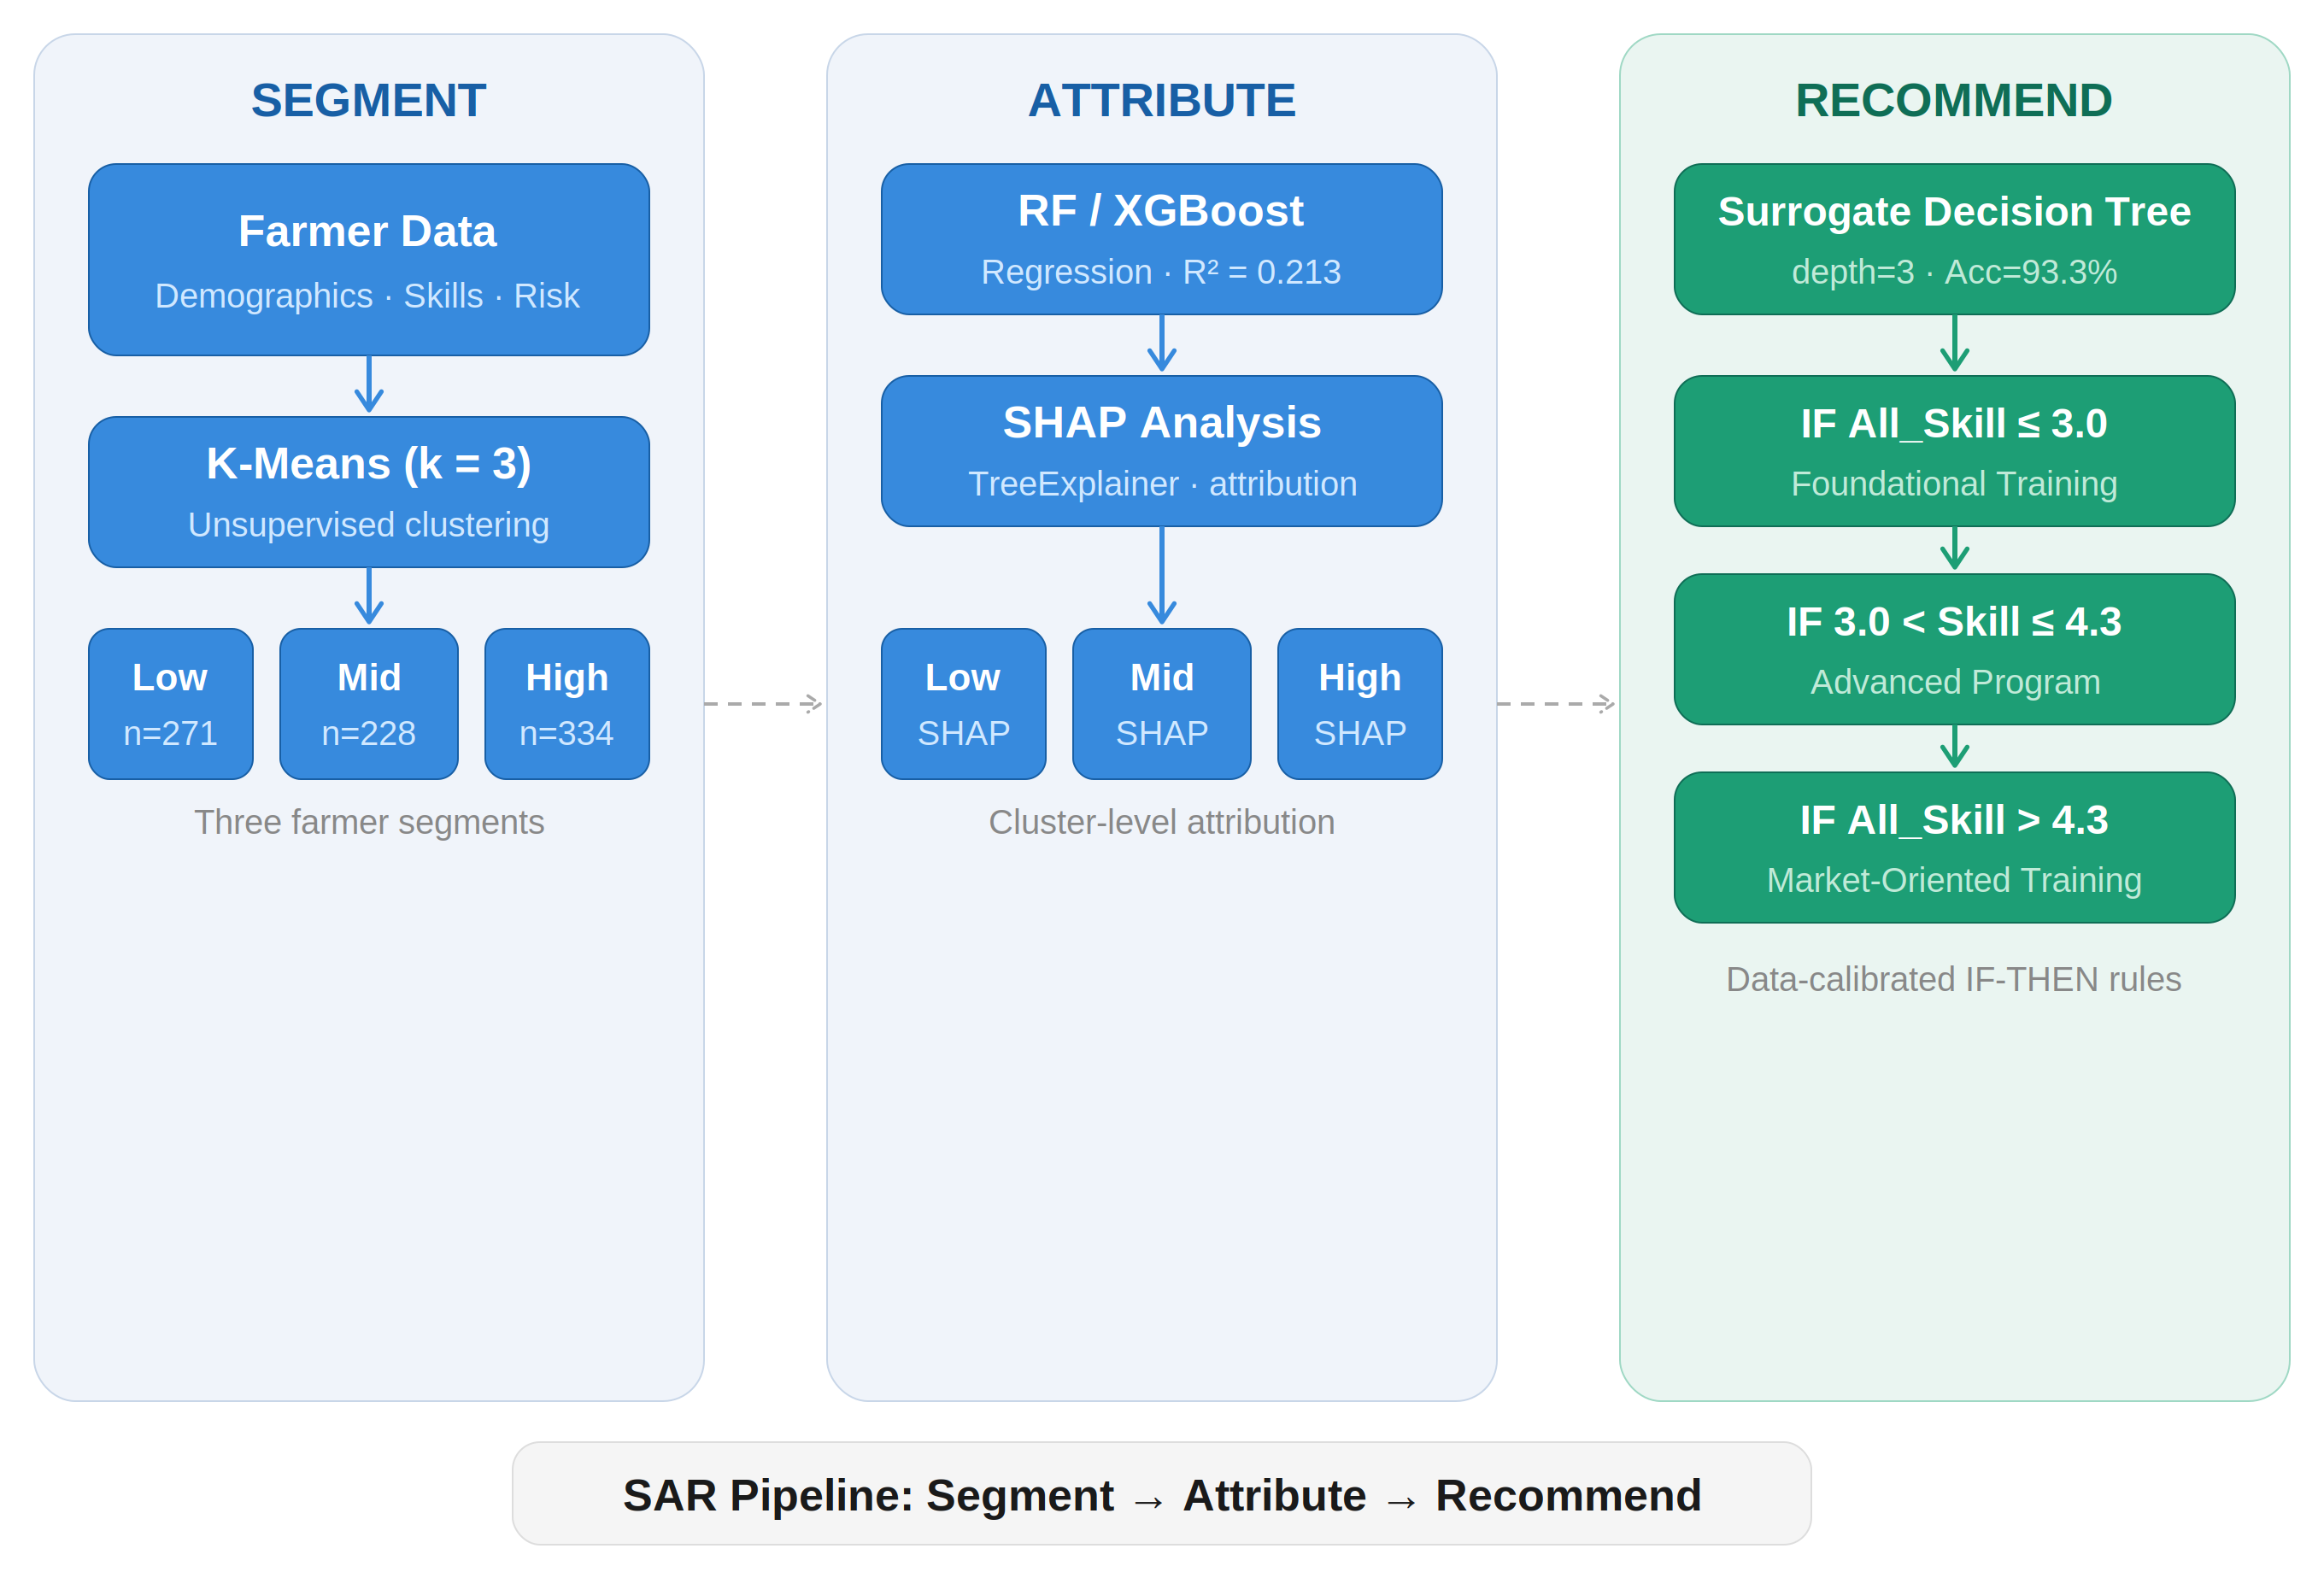
\includegraphics[width=\textwidth]{figures/fig1_framework.png}
\caption{SAR framework: three-stage pipeline (Segment, Attribute, Recommend) for interpretable allocation.}
\label{fig:framework}
\end{figure*}

\begin{figure}[htbp]
\centering

\includegraphics[width=\columnwidth]{figures/fig_elbow_silhouette.png}
\caption{Cluster validity across $k = 2$--$8$: Elbow, Silhouette, Calinski--Harabasz, and Davies--Bouldin.
At $k = 3$: Silhouette $= 0.185$, CH $= 202.67$, DB $= 1.835$.}
\label{fig:elbow}
\end{figure}

\begin{figure}[htbp]
\centering

\includegraphics[width=\columnwidth]{figures/fig2_clusters_new.png}
\caption{Population segmentation via K-Means ($k = 3$) in PCA space. Three clusters show different profiles.}
\label{fig:clusters}
\end{figure}

\begin{figure}[htbp]
\centering

\includegraphics[width=\columnwidth]{figures/fig_k_sensitivity.png}
\caption{K-sensitivity analysis: validity indices for $k = 2$--$5$. Segment structure remains consistent.
The segment structure remains consistent across values of $k$, supporting the robustness of the three-segment solution.}
\label{fig:sensitivity}
\end{figure}

\begin{figure}[htbp]
\centering
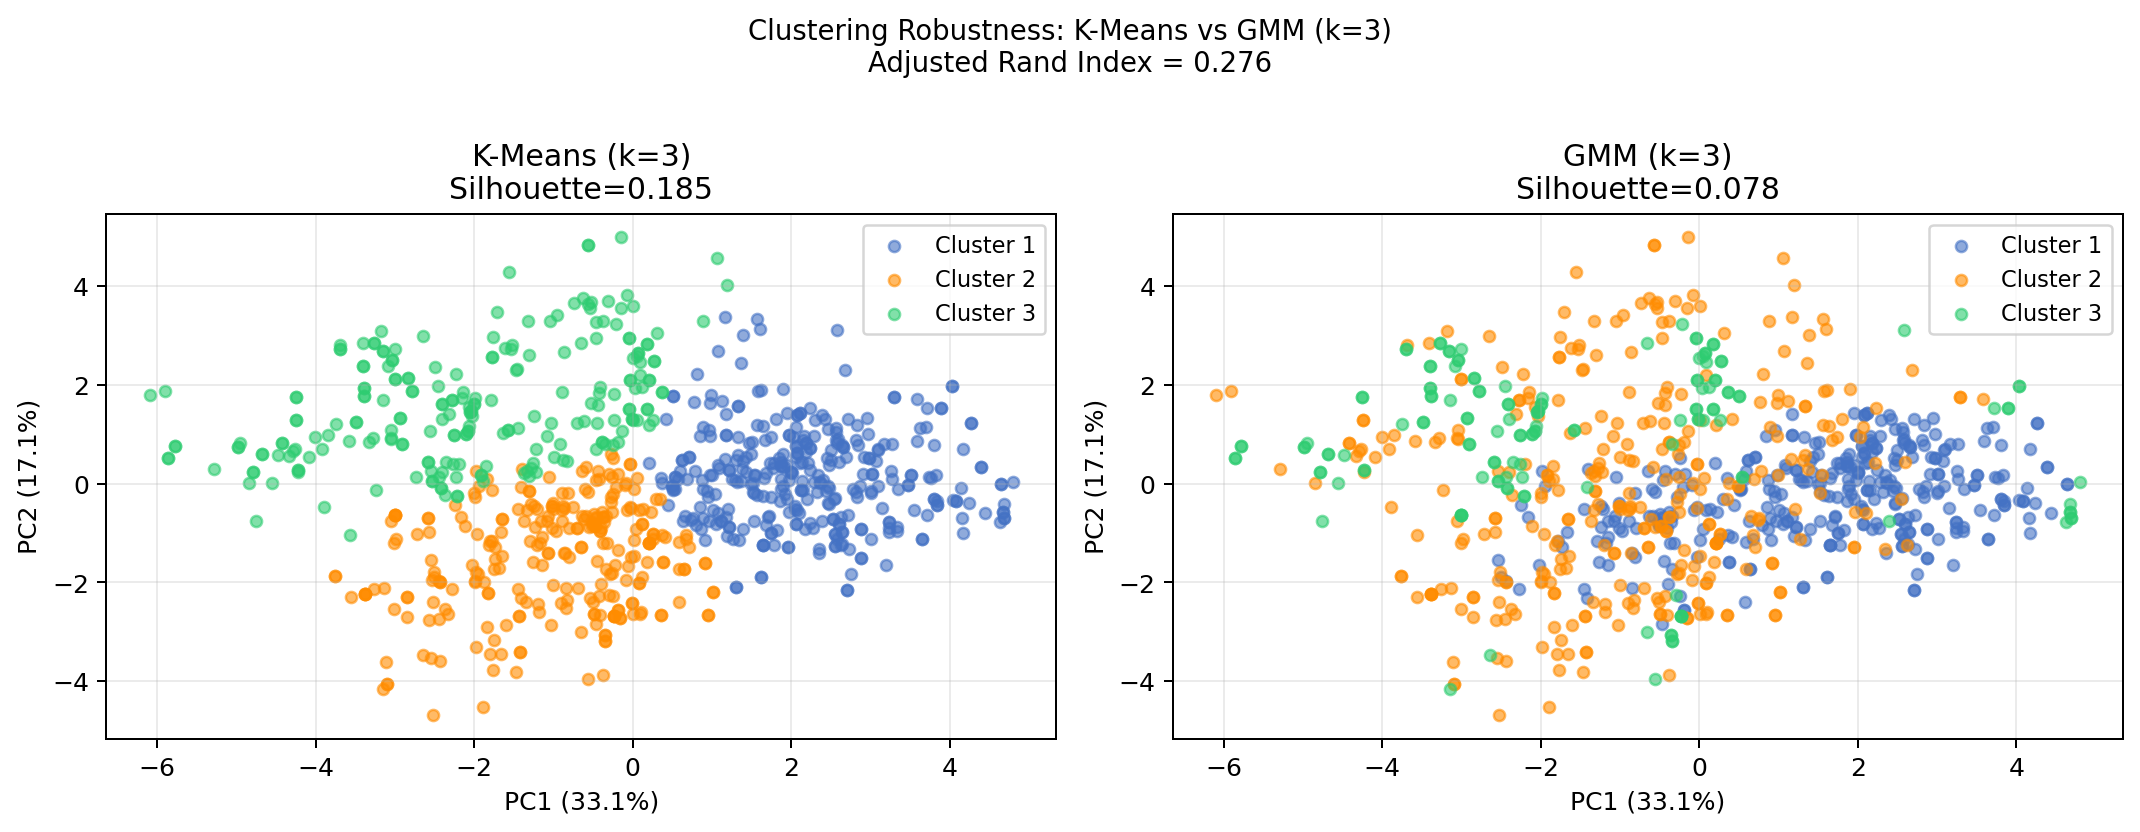
\includegraphics[width=\columnwidth]{figures/fig_gmm_robustness.png}
\caption{Clustering robustness: K-Means versus GMM ($k = 3$). Adjusted Rand Index = 0.28.
K-Means produces more balanced and interpretable segment groupings
than GMM in this Likert-scale dataset.}
\label{fig:gmm}
\end{figure}

\begin{figure}[htbp]
\centering

\includegraphics[width=\columnwidth]{figures/fig3_importance_new.png}
\caption{Global SHAP importance across all observations ($n = 833$). \texttt{All\_Skill} is the top driver.}
%\caption{Global SHAP importance across all observations ($n = 833$). All_Skill is the top driver.}
\label{fig:importance}
\end{figure}

\begin{figure}[htbp]
\centering

\includegraphics[width=\columnwidth]{figures/fig_shap_robustness.png}
\caption{SHAP robustness: RF vs. XGBoost ranking agreement ($\rho = 0.793$, $p < 0.001$).}
\label{fig:robustness}
\end{figure}

\begin{figure}[htbp]
\centering

\includegraphics[width=\columnwidth]{figures/fig4_shap_new.png}
\caption{SHAP beeswarm: feature contribution patterns ($n = 833$). Red = high, blue = low values.}
\label{fig:shap}
\end{figure}

\begin{figure*}[htbp]
\centering

\includegraphics[width=\textwidth]{figures/fig4b_cluster_shap_new.png}
\caption{Cluster-stratified SHAP: three segments show different feature patterns ($n = 271, 228, 334$).}
\label{fig:clusterShap}
\end{figure*}

\begin{figure*}[htbp]
\centering

\includegraphics[width=\textwidth]{figures/fig5_rules_new.png}
\caption{Surrogate decision tree (depth 3): in-sample accuracy 93.3\% ($n = 817$), held-out 91.4\%.
Node labels show the splitting feature, threshold, sample count,
and class distribution.}
\label{fig:rules}
\end{figure*}

%%─────────────────────────────────────────────────────────────────────────────
\section{Discussion}
%%─────────────────────────────────────────────────────────────────────────────

\subsection*{Predictive Performance}
Our Random Forest model achieved an $R^{2}$ of 0.283, which is consistent with other research on human learning.
 In these studies, outcomes are often influenced by factors we cannot measure, such as motivation and teacher quality. 

Our goal is not just to make the most accurate prediction, but to provide clear, actionable guidance. 
As shown by previous research, SHAP values are reliable for finding consistent patterns even when overall accuracy is moderate. 
The strong agreement between our Random Forest and XGBoost models ($\rho = 0.793$) confirms that 
our findings reflect real patterns rather than errors in our model. In the SAR framework, 
the model serves as a tool to translate complex data into simple, policy-ready guidelines.

\subsection*{Segment-Specific Drivers}
Our segment-level analysis shows that the factors driving skill growth differ across groups.
While starting skill level is the most important factor for everyone, other drivers vary. 

The slight decline in average skills for the Low- and Moderate-skill groups is common in these types of assessments. 
It is partly due to statistical factors like "regression-to-the-mean," but it also shows 
that farmers with lower initial engagement may not benefit from general training. Meanwhile, for the High-skill group, marketing skills are the key driver. This suggests that advanced farmers need training that focuses on market knowledge rather than basic production.

\subsection*{Practical Application}
Our surrogate decision tree achieved 93.3\% accuracy on the full dataset and 91.4\% on unseen data. 
This proves that our rules are reliable and not just "memorizing" the training data. 

The SAR framework offers a simple, four-step workflow: (1) record farmer background, (2)
 assign the farmer to a group, (3) apply the decision rules, and (4) provide a recommendation. 
 Because the rules are written in plain IF--THEN format, extension officers can use them without 
 needing to understand machine learning. This transparency is essential for public-sector programs 
 that must be accountable to the farmers they serve.

%%─────────────────────────────────────────────────────────────────────────────
\section{Conclusion}
%%─────────────────────────────────────────────────────────────────────────────

This study presents SAR, a practical decision support system for agricultural training allocation. By combining clustering, predictive modeling, and XAI, we have developed a framework that turns complex data into clear, actionable rules for extension officers.

Our findings show that while starting skill level is the strongest predictor of training success, the actual drivers of performance vary significantly across different groups of farmers. By using SHAP attribution within specific segments, we have identified these differences and converted them into simple IF--THEN rules that are both accurate and easy to use.

The high performance of our decision rules on unseen data demonstrates that the SAR framework is a robust tool for real-world policy deployment. Rather than focusing solely on predictive accuracy, we prioritized transparency and interpretability to ensure that our recommendations can be used directly in the field. 

Future work will focus on testing these rules in other regions, conducting controlled experiments to measure actual skill impact, and connecting the SAR pipeline to live data systems. We believe this framework provides a concrete, scalable path toward integrating explainable AI into agricultural extension programs.

%%─────────────────────────────────────────────────────────────────────────────
\section*{Acknowledgements}

This study was supported by the United States Agency for International Development (USAID) through the Department of Agricultural and Resource Economics, Faculty of Economics at Kasetsart University, in partnership with Michigan State University. The authors are deeply grateful to all survey respondents for their cooperation. We would like to thank Professor Mywish Maredia (Michigan State University) for her invaluable guidance and the officers of the Farmer Development Division at the Department of Agricultural Extension for their assistance in facilitating data access and providing program information. 

Additionally, this work was supported by the Research and Development Institute at Bansomdejchaopraya Rajabhat University under an internal research grant program dedicated to supporting faculty members in their pursuit of academic rank advancement.

\section*{Funding}
This research was supported by the United States Agency for International Development (USAID) through Michigan State University. Additional financial support was provided by the Research and Development Institute at Bansomdejchaopraya Rajabhat University under an internal research grant program for academic rank advancement.

\section*{Ethics Statement}
This study was reviewed and exempted by the Kasetsart University Research Ethics Committee (Approval No. COE67/044, issued on 8 May 2024). All procedures were performed in accordance with the ethical guidelines for human research.

\section*{Data and Code Availability}
The anonymised dataset used in this study is available upon reasonable request, subject to the existing data-sharing agreement with the Department of Agricultural Extension, Thailand. The complete SAR framework pipeline—including clustering, Random Forest training, SHAP attribution analysis, and surrogate rule extraction scripts—is maintained in a version-controlled repository. This repository will be made publicly available on GitHub upon acceptance of this manuscript to ensure full reproducibility of our results.

\section*{Declaration of Competing Interest}
The authors declare no competing interests.

\section*{Author Contributions}
\textbf{Kitti Chiewchan:} Conceptualisation, Methodology, Machine Learning Analysis, System Architecture Design, Writing -- Original Draft, Review \& Editing. \\
\textbf{Jumtip Seneerattanaprayul:} Questionnaire Design, Data Collection, Impact Evaluation (Difference-in-Difference analysis), Result Validation.

\section*{Declaration of Generative AI and AI-assisted technologies}
During the preparation of this manuscript, the authors used Generative AI models to assist with language refinement and structural formatting. All analytical decisions, algorithmic implementations, and substantive content were developed by the authors. The authors reviewed, edited, and verified all generated material and take full responsibility for the final content of the article.

% Bibliography style for natbib (adds \bibstyle/\bibdata equivalents)
\bibliography{sample}

\end{document}